\lecture{6}{11. September 2025}{Free-body diagrams and equilibrium equations 3D}


\subsection{Equations of equilibrium}
Above it is noted that the necessary and sufficient conditions for equilibrium for a rigid body is $\sum \textbf{F} = 0$ and $\sum \textbf{M}_O = 0$. In two dimensions this is often written as:
\begin{align*}
  \sum F_x &= 0 \\
  \sum F_y &= 0 \\
  \sum M_0 &= 0
.\end{align*}

Although the above representation is the most frequently used one, two alternate sets of three independent equilibrium equations may also be used. One of these is:
\begin{align*}
  \sum F_x &= 0 \\
  \sum M_A &= 0 \\
  \sum M_B &= 0
.\end{align*}
Here $M_A$ and $M_B$ is the moments about an arbitrary point $A$ and $B$, respectively. When applying these it is a requirement that a line passing through $A$ and $B$ is not parallel to the $y$-axis. 

Another set of equilibrium equations is:
\begin{align*}
  \sum M_B &= 0 \\
  \sum M_C &= 0
.\end{align*}
Here it is a requirement that points $A$, $B$, and $C$ do not lie on the same line.


\subsection{Two- and Three-force members}
The solutions to some equilibrium problems can be simplified by recognizing members that are only subjected to two or three forces.

\subsubsection{Two-Force Members}
A two-force member has forces applied at only two points. An example of this is shown on \autoref{fig:f4_16}. To satisfy force equilibrium, $\textbf{F}_A$ and $\textbf{F}_B$ must be equal in magnitude but opposite in direction. Furthermore, moment equilibrium requires that $\textbf{F}_A$ and $\textbf{F}_B$ share the same line of action, which can only happen if they are directed along the line joining $A$ and $B$. 

\begin{figure} [ht]
  \centering
  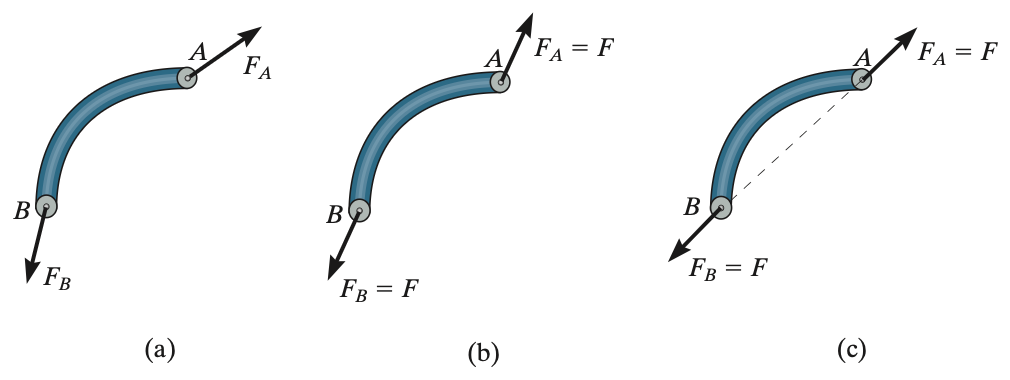
\includegraphics[width=0.5\linewidth]{./figures/f4_16.png}
  \caption{Two-force member}
  \label{fig:f4_16}
\end{figure}

\subsubsection{Three-Force Members}
A three-force member has forces applied at three different points. Moment equilibrium can only be satisfied if the three forces form a \textit{concurrent} or \textit{parallel} force system. These two cases are shown on \autoref{fig:f4_17}.

\begin{figure} [ht]
  \centering
  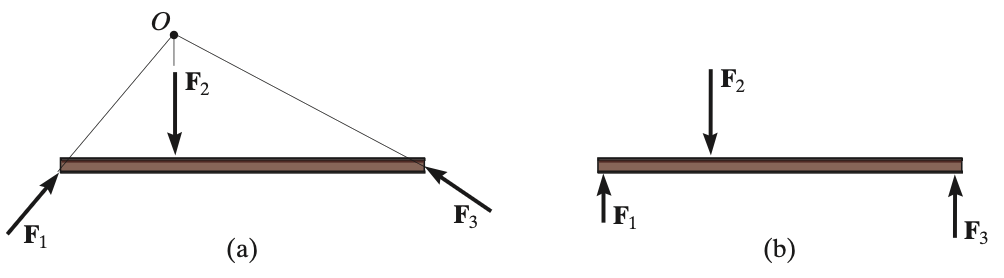
\includegraphics[width=0.5\linewidth]{./figures/f4_17.png}
  \caption{Three-force member}
  \label{fig:f4_17}
\end{figure}


\section{Equilibrium in Three Dimensions}

\subsection{Equations of Equilibrium}
In three dimensions the vector equations of equilibrium may be stated as:
\begin{align*}
  \sum \textbf{F} &= \textbf{0} \\
  \sum \textbf{M}_O &= \textbf{0}
.\end{align*}


In cartesian form this is:
\begin{align*}
  \sum \textbf{F} &= \sum F_x \textbf{i} + \sum F_y \textbf{j} + \sum F_z \textbf{k} = \textbf{0} \\
  \sum \textbf{M}_O &= \sum M_x \textbf{i} + \sum M_y \textbf{j} + \sum M_z \textbf{k} = \textbf{0} 
.\end{align*}
This can be broken down into six scalar equations, which may be used to solve for at most six unknowns.
